\documentclass[letterpaper, 12pt]{article}

%%%%%%%%%%%%%%%%%%%%%%%%%%%%%
% DEFINITIONS
% Change those informations
% If you need umlauts you have to escape them, e.g. for an ü you have to write \"u
\gdef\mytitle{Ausarbeitung}
\gdef\mythema{Synchronisierung \& Konsistenz}

\gdef\mysubject{SYT}
\gdef\mycourse{5BHIT 2015/16}
\gdef\myauthor{Erik Br\"andli \& Michael Weinberger}

\gdef\myversion{1.0}
\gdef\mybegin{6. November 2015}
\gdef\myfinish{23.02.2016}

\gdef\mygrade{}
\gdef\myteacher{}
%
%%%%%%%%%%%%%%%%%%%%%%%%%%%%%

\input special/preamble.tex

\let\tempsection\section
\renewcommand\section[1]{\vspace{-0.3cm}\tempsection{#1}\vspace{-0.3cm}}
\WithSuffix\newcommand\section*[1]{\tempsection*{#1}}

\let\tempsubsection\subsection
\renewcommand\subsection[1]{\vspace{0cm}\tempsubsection{#1}\vspace{0cm}}

\let\tempsubsubsection\subsubsection
\renewcommand\subsubsection[1]{\vspace{0cm}\tempsubsubsection{#1}\vspace{0cm}}

\linespread{0.94}

\lhead{\mysubject}
\chead{}
\rhead{\bfseries\mythema}
\lfoot{\mycourse}
\cfoot{\thepage}
% Creative Commons license BY
% http://creativecommons.org/licenses/?lang=de
\rfoot{\ccby\hspace{2mm}\myauthor}
\renewcommand{\headrulewidth}{0.4pt}
\renewcommand{\footrulewidth}{0.4pt}

\begin{document}
\parindent 0pt
\parskip 6pt

\pagenumbering{Roman} 
%!TEX root=../laborprotokoll.tex

\begin{titlepage}

	\begin{figure}[!h]
		\begin{flushright}
			
\includegraphics[width=0.3\linewidth]{images/jdIT_tgm.png}
		\end{flushright}
	\end{figure}

	\vspace{2.5cm} 

	{\begin{center} \bfseries\huge
			\rule{17.5cm}{0.1mm}  
			\\[5mm]
			\mytitle\\[5mm]
			\mythema\\
			\rule{17.5cm}{0.1mm}  
	\end{center}}

	{\begin{flushright} \bfseries\Large
			\vspace{2cm}
			\mysubject\\
			\mycourse\\[10mm]
			\myauthor\\[10mm]
	\end{flushright}}

	{\begin{table}[!h] \bfseries\normalsize
		\begin{tabularx}{\textwidth}{lXr @{\hspace{0mm}}}
			&& Version \myversion\\
			\mygrade && Begonnen am \mybegin\\
			\myteacher && Beendet am \myfinish\\
		\end{tabularx}
	\end{table}}

\end{titlepage}


\clearpage
\thispagestyle{empty}
\tableofcontents

\newpage
\pagenumbering{arabic}
\pagestyle{fancy}

%\vspace{-0.5cm}
\section{Disaster Recovery}

\subsection{Grundlagen \& Definitionen \cite{bookone} \cite{intro} \cite{intro2} \cite{intro3} \cite{downtime}}
Disaster Recovery (dt. auch Katastrophenwiederherstellung), im Folgenden auch \textit{DR} genannt, beschreibt die Vorbereitung und Reaktion auf sogenannte Katastrophen, die abgespeicherte Daten und Lauffähigkeit eines IT-Systems betreffen. In diesem Bereich der Sicherheitsplanung ist mit negativen Ereignissen all das gemeint, was den Betrieb eines Unternehmens gefährdet. Hierzu gehören Cyberattacken, Infrastrukturausfälle ebenso wie Naturkatastrophen. DR umfasst beispielsweise Schritte zur Wiederherstellung von Server oder Mainframes mit Backups oder ferner die Bereitstellung von LANs für die unmittelbaren geschäftlichen Bedürfnisse. \\

Anhand einiger Beispiele von Oxford Knowledge wird die Sinnhaftigkeit der Technologie bewiesen:

\begin{itemize}
	\item 93\% der befragten Firmen, die ihre Datenzentren für 10 oder mehr Tage aufgrund eines Desasters nicht erreichen konnten, mussten innerhalb eines Jahres nach dem erstmaligen Auftreten Konkurs anmelden.
	\item Im Vereinigten Königreich wurden 70\% der befragten Firmen, die einen großen Datenverlust verzeichneten innerhalb von 18 Monaten geschlossen.
	\item 29\% der befragten Firmen hatten bereits mit Systemausfällen und korrumpierten Daten zu tun.
	\item 52\% der befragten Firmen wurden bereits Opfer einer (gelungenen/nicht gelungenen) Cyberattacke.
\end{itemize}

\subsubsection{Disaster Recovery Plan}

In dessen Folge dokumentiert ein Disaster Recovery Plan, im Folgenden auch DRP genannt, dann konkret Richtlinien, Verfahren und Maßnahmen, um die Störung eines Unternehmens im Falle eines Desasters zu begrenzen, und möglichst innerhalb eines bestimmten Zeitrahmens wieder zurück zum Normalzustand überzugehen. Wie bei einer Katastrophe macht das Ereignis die Fortführung des normalen Geschäftsbetriebs unmöglich. Genannter Plan sollte ein Teil eines jeden Standard-Projektmanagementsprozess sein. \\
Falls ein DRP besteht, kann das Unternehmen die Auswirkungen des Desasters minimieren und ihre geschäftskritischen Prozesse schnell fortführen. Die Disaster-Recovery-Planung beinhaltet in der Regel eine Analyse der Geschäftsprozesse und des Bedarfs. Sie kann auch einen Schwerpunkt zur Prävention beinhalten. Disaster Recovery ist ein wichtiger Aspekt von Enterprise-Computing. Die Unterbrechung des Dienstes oder der Verlust von Daten kann sich schwerwiegend auf die Finanzen auswirken, sei es direkt oder durch den etwaigen darauffolgenden Imageverlust. \\
Die internationale Norm für Sicherheitsmanagement erlangt immer mehr Aufmerksamkeit, da viele größere Organisationen ihre IT-Service-Provider \textbf{ISO27001}-konform machen.

\newpage

\subsubsection{Business Continuity}

Business Continuity, dt. Betriebliches Kontinuitätsmanagement, beschreibt Prozesse und Verfahren eines Unternehmens, die die Weiterführung von wichtigen Geschäftsprozessen während und nach einem Desaster sichern sollen. Dabei liegt der Schwerpunkt mehr auf der Aufrechterhaltung der Geschäftstätigkeit als bei der Infrastruktur. Business Continuity und Disaster Recovery sind eng verbunden, sodass beide Begriffe manchmal kombiniert werden. \\
Die aufkommende internationale Norm für Business Continuity Management ist die \textbf{BS25999}. \\

\subsubsection{Was ist eigentlich eine Katastrophe?}

Wie bereits kurz erwähnt, eine Katastrophe kann vielerlei Ausmaß haben. Jede einzelne davon hat primäre und sekundäre Auswirkungen, die sich in direkte Schäden, korrumpierte oder unzugängliche Daten niederschlägt. Das eigene IT-Netzwerk ist verschiedensten Gefahren ausgesetzt, die in den schlimmsten Fällen auch ohne jegliche Vorwarnung auftreten können. \\
Einige Beispiele:

\begin{itemize}
	\item Feuer, Brand im Serverraum, Wasserrohrbruch
	\item Sonstige Naturkatastrophen \\ Sind ebenso zu berücksichtigen, speziell bei hoher Sicherheitsstufe!
	\item Sicherheitsprobleme, Viren, Cyberattacken, Datendiebstahl
	\item Hardware- und Softwareausfälle
	\item Stromausfall
	\item ...
\end{itemize}

Die Liste könnte noch weiter fortgeführt werden, wichtig ist, dass möglichst alle wichtigen und für die Umgebung relevanten Faktoren berücksichtigt werden. Kleinere Disaster treten immer häufiger bzw. mit einer größeren Wahrscheinlichkeit auf. \\
So fern es sich anhört, Naturkatastrophen haben wenn sie auftreten die verheerendste Auswirkung. Unter einer Aktiv/Aktiv-Konfiguration versteht man in diesem Zusammenhang, dass die so gesicherte Ressource, also zum Beispiel eine Datenbank, auf allen Clusterknoten aktiv ist. Wenn ein Knoten ausfällt, übernehmen die übrigen Knoten die Prozesse des ausgefallenen Knotens, es gibt praktisch keinerlei Ausfallzeiten, eventuell jedoch starke Einbußen in der Performance, da die gleiche Last nun von weniger Systemen übernommen werden muss.

\begin{figure}[h]
    \subfigure[Risikofaktoren \cite{bild2}]{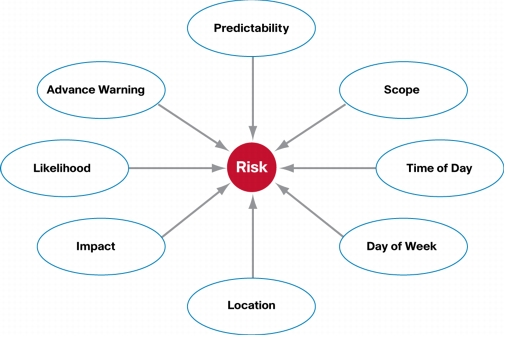
\includegraphics[width=0.49\textwidth]{images/white_paper_c11-453495-2.jpg}} 
    \subfigure[Extrembeispiel Erdbeben \cite{bild3}]{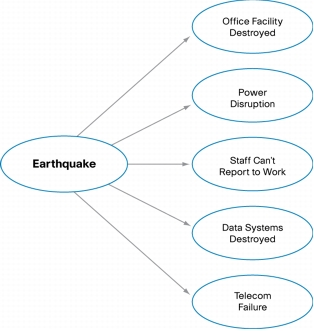
\includegraphics[width=0.49\textwidth]{images/white_paper_c11-453495-3.jpg}} 
\caption{Katastrophe \& Auswirkung, Risikoabschätzung} 
\end{figure} 
\newpage

\subsubsection{Problem der Downtime, Kosten, max. Häufigkeit}

Das Beispiel des Webblogs 'Interxion' zeigt mögliche Kosten bei einem internationalen Marktführer wie etwa Facebook: \\
Als Facebook am 1. August 2014 großteils nicht erreichbar war, riefen hunderte amerikanischer Nutzer ihren nächstgelegenen Polizeiposten an. Die Downtime dauerte zwar nur 20 Minuten, soll das Unternehmen aber immerhin 500.000 \$ gekostet haben. Berechnet hat dies 'The Wire' aufgrund der Werbeeinnahmen von Facebook, die im Jahr 2,91 Milliarden \$ betragen – oder 22.453 \$ pro Minute. Es wird geschätzt, dass die wahren Kosten eines solchen Ausfalls weit höher liegen. Heikel dabei ist der Ruf des Unternehmens: Nicht nur Nutzer, auch diejenigen, die den Dienst finanzieren – die Werbetreibenden – bauen auf dessen Zuverlässigkeit. Jeder Nutzer, der wegen einer Downtime Facebook unfreiwilig den Rücken kehrt, bedeutet für die Werber ein verlorenes Mitglied ihrer Zielgruppe. In einer aktuellen Studie schätzen Unternehmen ihre Kosten für eine Stunde Ausfallzeit auf mindestens 20.000 \$, 20\% der Unternehmen auf über 100.000 \$. Natürlich spielt es eine Rolle, in welcher Branche das Unternehmen tätig ist, und wieviele Zugriffe auf Ihre Services erfolgen. Die Kostenberechnung für eine Server-Downtime ist ein komplexes Unterfangen –  nur den Verlust der Werbeinnahmen in Betracht zu ziehen, wie es im Fall Facebook gemacht wurde, greift sicher noch zu wenig weit.

\newpage

\subsubsection{Fehlertoleranz}

Jeder, der mit IT-Systemen arbeitet wurde auch schon Zeuge eines Ausfalls einer Komponente oder eines Service, wichtig ist auch, auf den Begriff Fehlertoleranz zu achten. \textit{Fehlertoleranz} ist die Möglichkeit des Systems, selbstständig und automatisch auf verschiedenste Bedingungen zu reagieren und dementsprechend auszugleichen. Durch das selbsständige Vorgehen reduziert die Fehlertoleranz die Auswirkungen auf das System. Das System, das Programm, der Prozess wird weiterlaufen, vollkommen unbewusst, das ein Problem aufgetreten ist. Abhängig des Fehlertoleranzgrads des eingesetzten Systems müsste ein DRP in der Theorie gar nicht nötig sein, die Praxis spiegelt jedoch ein anderes Bild wieder. Wichtige Systeme haben einen höheren Fehlertoleranzgrad als weniger wichtige, wo nicht jeder Fehler zu einem schwerwiegenden Problem werden darf. Hohe Fehlertoleranz ist jedoch auch mit hohen Kosten verbunden.

\subsection{Aufstellen eines DRP \cite{booktwo}}

Ein Disaster Recovery Plan muss Desasteridentifikation, Kommunikationsrichtlinien, 
das Koordinieren der Prozesse, etwaige Ausweichmöglichkeiten, Prozesse, um so schnel wie möglich wieder 
zum Normalzustand zurückzukehren und einen Feldtest des Plans sowie Wartungsroutinen beinhalten. 
Es muss kurz ein funktioneller Plan sein, der alle Prozessketten richtig adressiert, um die 
Systeme wiederherzustellen, inkl. eines Zuständigen zur stetigen Wartung des Plans.
Es empfiehlt sich außerdem ein eigenes Disaster Response-Team auszuweisen, abhängig von den
gegebenen Anforderungen. Wenn der Plan entworfen wird, ist es wichtig eine Priorisierung aufzustellen,
welche Infrastruktur bzw. Systeme für den Erhalt der Einsatzfähigkeit zwingend nötig sind. Ein erstes Maß
ist die Wiederherstellung der voraussetzenden Umgebungen, etwa ein funktionierendes internes Netzwerk. Ein 
zweiter Punkt ist die auferlegte nötige Uptime für jedes System. Diejenigen, die eine 24/7-Uptime erreichen sollen
sind den weniger prioren vorzuziehen.
Es ist auch zu bedenken, dass bestimmte Workarounds effektiv laufen sollen, ohne noch größere Probleme
zu verursachen. Der Ersteller des Plans muss möglichst viele Daten sammeln über alle verwendeten Systeme,
sowie Abhängigkeiten untereinander abbilden und miteinander in Konflikt stehende, gleichrangige Priorisierungen klären. Ein DRP wird nicht automatisch ausgeführt, sondern händisch, angepasst an den Bedarfsfall.

\subsection{Schaffung eines zuverlässigen Systems \cite{bookthree}}

\subsubsection{Clustersysteme und deren Vorteile}

Wenn Systeme 24/7 verfügbar sein müssen, wird oft eine Clusterlösung herangezogen. Hier unterscheidet man zwischen zwei Varianten, Failover-Clustering und 'echtem' Clustering. Bei der Failover-Technologie mit zwei oder mehreren Netzwerkdiensten übernimmt ein Zweitsystem bei einseitigem Ausfall des Primärsystems. Echtes Clustering, sprich ein Aktiv/Aktiv-Cluster, wird bezeichnet einen Rechnerverbund, in dem mehrere (meistens > 2) Nodes gleichzeitig aktiv sind. Computercluster werden neben der Verteilung der Rechenleistung auch u. a. zur Sicherstellung der Verfügbarkeit von diversen Ressourcen wie Netzwerke, Applikationen etc. verwendet. Unter einer Aktiv/Aktiv-Konfiguration versteht man in diesem Zusammenhang, dass die so gesicherte Ressource, also zum Beispiel eine Datenbank, auf allen Clusterknoten aktiv ist. Beide Herangehensweisen beinhalten keinen DRP. Da sie '100\% der Zeit' verfügbar sind (aus Sicht des Kunden), gibt es per se keine Katastrophen, die die Business Continuity beeinträchtigen. Der einzige Nachteil: Solche Lösungen sind meistens sehr teuer in Aufbau und Wartung, und daher eher nur von großen Unternehmen mit großem Budget zu bewerkstelligen.

\subsubsection{Wieso dann DR?}

Für Systeme, die keine 100\%-ige Verfügbarkeit benötigen, oder das Budget es nicht anders vorsieht, ist DR die bessere Wahl. Eine typische Lösung ist es ein identes System aufzubauen, es für etwaige Einsatzfälle zu warten und es als Failover zu verwenden. Der Wechsel auf dieses System verlangt einen Eingriff des Administrators, während dieser Zeit bis zur Inbetriebnahme 'steht der Betrieb'. Die Rückkehr auf den Normalzustand kann mithilfe dieser Methode relativ schnell wiedererlangt werden, und generiert weniger Kosten als eine vollständige Cluster-Lösung. \\
Die billigste Variante (aus Hardware-Sicht) ist es auf Fehler zu reagieren, nachdem sie passiert sind. Hier wird das gesamte System heruntergefahren bis der Fehler ausgebessert ist, der Betrieb kann nicht fortgeführt werden. Wenn z.B. die Festplatte ausfällt, steht die gesamte Infrastruktur still, bis einzig und allein die kaputte Festplatte ausgetauscht ist. Systemadministratoren können wie erwähnt Katastrophen nicht vollständig verhindern - sie können jedoch bestimmte Wahrscheinlichkeiten verringern und mit einem guten DRP komplette Wiederherstellungen gewährleisten mit einem Minimum an Zeit in einem geordneten Prozess. \\
Der Grad einer guten Absicherung hängt wie gesagt auch mit en Finanzen zusammen, in eine unterbrechungsfreie Stromversorgung (USV) sollte auf jeden Fall investiert werden. Die USV hält die Infrastruktur lang genug am Leben, um Files zu speichern und die Server sicher herunterzufahren, ein Strom-Backup ist wohl für kein System unwichtig. Fehlende Elektrizität ist nämlich die wohl wichtigste, weil häufigste Fehlerursache. \\
Eine regelmäßige Backup-Routine (täglich, wenn nicht sogar mehr) ist der Schlüssel zu einer erfolgreichen Katastrophenwiederherstellung. Ein Teil der Backups sollte an einem sicheren Platz abgelegt sein, wenn möglich außerhalb des eigenen Infrastruktur-Netzes. \\
Auch Redundanz spielt eine tragende Rolle beim Aufbau eines zuverlässigen Systems. Gute DR-Pläne sehen nicht vor, dass wichtige Daten jediglich auf einer Maschine liegen. Ohne diese Maßnahme wäre es nicht möglich, einen Failover-Server mit einer Kopie der kritischen Daten bereitzustellen. \textit{RAID} (Redundant Array Of Independent Disks) ist eine gute Lösung, um dem entgegenzuwirken. Hier haben, je nach Modus, mehrere Festplatten dieselben Daten. RAID ist ein zuverlässiger Schutz bei Datenträgerausfall, der ja bekanntlich eine 100\%-ige Wahrscheinlichkeit mit sich bringt. Die besten Umsetzungen erlauben sogar Hot-Swapping, damit ein Ersatz eingefügt werden kann, ohne dass das System eine Downtime erleidet. RAID bietet auch einen schnelleren Zugriff auf Daten, macht es u. a. effizient für Fileserver. 

\subsection{Disaster Recovery: Techniken \cite{traddr} \cite{traddr2}}

\subsubsection{Traditional Disaster Recovery}

\textit{SHARE} ist ein ehrenamtlicher Userzusammenschluss mit Fokus auf IBM-Systeme und -Technologien, und wurde bereits im Jahr 1955 gegründet. SHARE hat ursprünglich die \textit{Seven tiers of disaster recovery} definiert, um verschiedene Herangehensweisen zu beschreiben, um eben auftragskritische Computersysteme wiederherzustellen, und wurde darin auch von IBM selbst unterstützt. Obwohl das Originalkonzept bis in die späten 1980er-Jahre zurückreicht, verwenden DRP-Experten diesen Ansatz bis heute sehr häufig (Stand: Dez. 2015), um Möglichkeiten und Kosten darzustellen. Natürlich wurden die genauen Definitionen dementsprechend angepasst, um heutigen Standards besser zu entsprechen. \\
Das SHARE Technical Steering Committee in Zusammenarbeit mit IBM hat die Stufen (Tiers) auf die Zahlen 0 bis 6 festgelegt. Durch den technischen Fortschritt der vergangenen Jahrzehnte wurde eben eine 7. Stufe hinzugefügt, die mehrere auch geographisch voneinander unabhängige Systeme berücksichtigt, welches das höchste Maß an Verfügbarkeit darstellt. \\
Wie auch hier sind die aufkommenden Kosten von niedrig (Tier 0) bis hoch (Tier 7) gestaffelt.

\begin{figure}[h]
	\begin{center}
		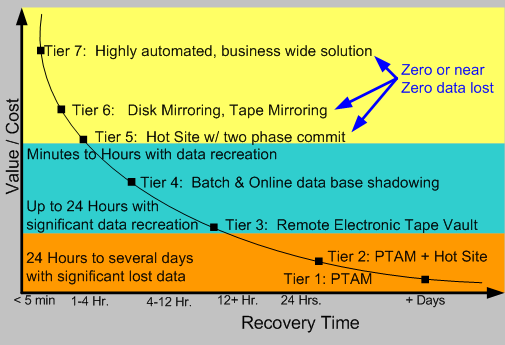
\includegraphics[width=0.6\linewidth]{images/7-tier}
		\caption{Seven tiers of disaster recovery \cite{bild1}}
		\label{Seven tiers of disaster recovery}
	\end{center}
\end{figure}

	\subsubsection{Tier 0: No off-site data – Possibly no recovery}
	Unternehmen mit einer Tier 0-Lösung haben keinen Disaster Recovery Plan. Sie haben keine gespeicherten Informationen über das System, keine Dokumentation und auch keine Backups. Die Zeit, die benötigt wird um ein solches System wiederherzustellen ist unvorhersehbar, es kann sogar sein, dass es unmöglich ist zum Normalzustand zurückzukehren.
	\subsubsection{Tier 1: Data backup with no hot site}
	Tier 1-Systeme erhalten regelmäßig ein Backup, und lagern diese an einem sicheren Ort, der sich außerhalb des eigenen Hauses (der eigenen Infrastruktur) befindet. Dies ist notwendig, da vor einem Desaster auch Backups mit lokalem, nicht redundanten Speicherort nicht sicher sind. Diese Methode Backups zu transportieren heißt PTAM, ausgeschrieben 'Pick-up Truck Access Method'. Sprich, das Backup ist so schnell greifbar, wie der Transport vom Aufbewahrungsort dauert. Abhängig davon, wie oft Sicherungen gemacht und versendet werden müssen Unternehmen einige Tage bzw. Wochen Datenverlust inkaufnehmen, dafür sind die Sicherungsdateien geschützt außerhalb des Geländes aufbewahrt.
	\subsubsection{Tier 2: Data backup with a hot site}
	Bei Verwendung von Tier 2 werden ebenso regelmäßige Sicherungen vorgenommen, auf langlebigen Speichermedien wie etwa Tapes. Das wird kombiniert mit eigener Infrastruktur außerhalb des eigenen Geländes (genannt 'Hot Side'), von welchen die Backups rückgelesen werden im Falle eines Desasters. Diese Lösung benötigt immer noch einige Stunden oder Tage zur Wiederherstellung, jedoch ist die Gesamtdauer besser vorhersehbar.
	\subsubsection{Tier 3: Electronic vaulting}
	Der Ansatz Tier 3 baut auf Tier 2 auf. Hinzufügend dazu werden kritische Daten elektronisch abgekapselt von den weniger prioren. Die Abgekapselten sind üblicherweise aktueller als die Daten, die via PTAM abgelegt werden. Als Ergebnis ist hier weniger Dateiverlust, sollte eine Katastrophe eintreten. \\ Einrichtungen, die 'Electronic Remote Vaulting' bereitstellen, verfügen über Hochgeschwindigkeitsanbindungen und entweder physische oder virtuelle Sicherheitstape-Lesegeräte, mit automatisierter Sicherungsbibliothek beim entfernten Standort. \\ Als praktischen Beispiel zur Implementierung dienen IBMs Peer-to-Peer TotalStorage Virtual Tape Server oder Oracles VMS Clustering.
	\subsubsection{Tier 4: Point-in-time copies}
	Tier 4-Lösungen werden oft von Unternehmen verwendet, die hohen Wert auf Datenkorrektheit und schneller Wiederherstellung legen als die unteren Stufen bereitstellen. Eher als das Auslagern von Speichertapes wie bei 0-3 gegeben, integriert diese Stufe Sicherungen auf Basis von Disks (also Festplatten). Immer noch sind mehrere Stunden Datenverlust möglich, jedoch ist es einfacher Point-in-Time-Backups (PiT, jeweils zu einem festgelegten Zeitpunkt) zu erstellen mit einer höheren Frequenz als Tape-Sicherungen, sogar wenn elektronisch gekapselt.
	\subsubsection{Tier 5: Transaction integrity} 
	Tier 5 wird verwendet, wenn es zwingend erforderlich ist, dass Daten konsistent sind zwischen Produktivsystem und dem Wiederherstellungs-Remoteserver. Bei einem solchen Aufbau kommt es zu kaum bis gar keinem Datenverlust, aber die Verfügbarkeit dieser Funktionalität ist stark abhängig von der verwendeten Implementierung.
	\subsubsection{Tier 6: Zero or near-Zero data loss} 
	Tier 6 hält das höchste Maß an Datenrichtigkeit aufrecht. Dieser Ansatz wird eingesetzt von Systemen, in denen wenig oder gar kein Datenverlust vertretbar ist, und wo Daten für den weiteren Gebrauch schnell wiederhergesellt werden müssen. Solche Lösungen haben keine Abhängigkeit von Anwendungen oder Mitarbeitern, um Datenkonsistenz zu gewährleisten. \\
	Tier 6 erfordert eine Form von Disk Mirroring zu einem Remoteserver, hierfür gibt es verschiedenste synchrone oder asynchrone Implementierungen von vielen Herstellern. Jede Herangehenweise ist leicht anders, mit verschiedenen Möglichkeiten und anderen Recovery Point/Recovery Time-Anforderungen. In den manchen Fällen wird jedoch auch eine Art von Tape-Speicherung benötigt, abhängig von dem erforderlichen Speicherplatz, der von Backup in Anspruch genommen wird.
	\subsubsection{Tier 7: Highly automated, business integrated solution} 
	Das höchste Level nimmt all die Hauptkomponenten von Tier 6 zusammen und fügt die Intgration von Automation hinzu. Das erlaubt Tier 7 damit auch die Datenkonsistenz, die bei Tier 6 gegeben ist. Desaster werden automatisch erkannt von Geräten außerhalb des eigenen Computersystems. Außerdem wird die Wiederherstellung automatisch ausgeführt, was sozusagen den kompletten Wiederherstellungsprozess bei System und Anwendungen beschleunigt, und diese schneller und zuverlässiger laufen lässt als es überhaupt möglich wäre durch händische Prozeduren. Die Ausfälle belaufen sich auf wenige Minuten oder Sekunden.
	
\subsubsection{Recovery Objectives}
Um die richtige Lösung zu erfassen, auch wenn Kosten ein Kriterium sind, bedarf es einer Evaluierung nach RTO/RPO.

\begin{itemize}
	\item Recovery Time Objective \\
	Beschreibt die Zeit, in der die Unternehmensfunktionen oder die Anwendungen spätestens wiederhergestellt sein sollen (inkludiert auch die Zeit, bis Vorgehensweisen bewertet, sowie die Zeit, um dann die nötigen Tasks abzuarbeiten)
	\item Recovery Point Objective \\
	Beschreibt wiederum die Zeit, die es maximal brauchen darf, bis genug Daten wiederhergestellt sind, um den Unternehmensprozess fortführen zu lassen.
\end{itemize}

Es sind viele Lösungen verfügbar, die richtige auszuwählen bedarf einer Kosteneinschätzung sowie auch hier die vertretbare Downtime und das Maß an Datenverlust abzuwägen. Etwa ist ein wenig Datenverlust akzeptierbar, wenn diese aus anderen Quellen leicht wiederhergestellt oder gar neu generiert werden können. \\ Es gibt keine Eine-für-alle-Lösung, der beste Ansatz ist vielleicht eine Mischung der oben genannten Stufen. Auf diesem Wege kann günstig das richtige Level an Schutz umgesetzt werden. Eine vorgefertigte einzelne Lösung oder Herangehensweise ist bei weitem nicht die beste Wahl.

\subsection{Disaster Recovery as a Service (DRaaS) \cite{draas}}
Oft auch nur \textit{Recovery as a service} genannt, ist DRaaS eine Unterkategorie des Cloud Computings und eine zuverlässige Form des Disaster Recovery. Es grenzt sich von cloudbasierten Backups ab, indem es auch bestimmte Daten schützt und auf Abruf Rechenkapazität bereitstellt, um die Wiederherstellung zu beschleunigen und als Failover zu dienen. Als Teil des Cloud Computing-Modells folgt es dem Prinzip, dass nur das bezahlt werden muss, was man auch verwendet hat. Damit kommt klar der Vortei zu tragen, dass traditionelle 'Warm Site'- oder 'Hot Site'-Aufbauten wesentlich ineffizienter sind, da sie ständig laufen und bezahlt werden müssen. \\
RaaS ist Teil der üblichen Nomenklatur, wie etwa IaaS, PaaS oder SaaS 

\begin{figure}[h]
	\begin{center}
		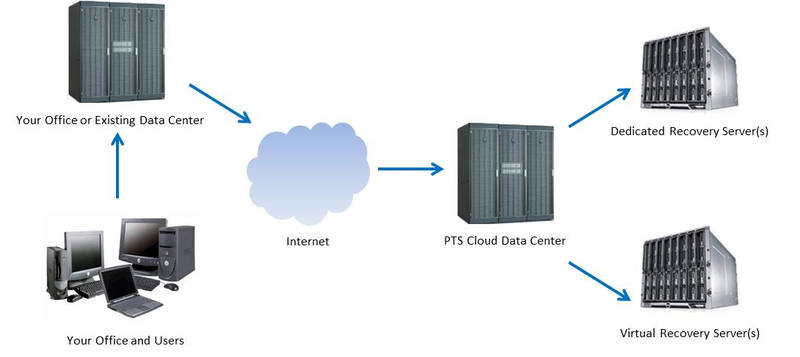
\includegraphics[width=1\linewidth]{images/disaster-recovery-as-a-service}
		\caption{Stark vereinfachte Darstellung von DRaaS \cite{bild4}}
		\label{DRaaS}
	\end{center}
\end{figure}

\subsubsection{Architekturen}

\begin{itemize}
	\item To-Cloud RaaS \\
	Die Zielanwendung befindet sich im primären, privaten Datencenter, und die Cloud wird als Backup- und Recovery-Target verwendet.
	\item In-Cloud RaaS \\
	Bedeutet, dass sowohl Zielanwendung als auch Recovery-Sites in der Cloud angesiedelt sind.
	\item From-Cloud RaaS \\
	Die Primärdaten liegen in der Cloud, und das Backup-Target liegt im privaten Datencenter.
\end{itemize}

\subsubsection{Möglichkeiten einer Sandbox}

Sandboxes sind ein weit verbreiteter Bestandteil von RaaS-Lösungen. Eine Sandbox ist ein Pool an Infrastruktur mit einer Kopie der RaaS-geschützten Daten oder der jeweiligen Anwendung wo diese aufgesetzt und getestet werden können. Diese Kopie ist vom restlichen Netzwerk getrennt, nur der Systemadministrator hat darauf Zugriff. Ohne das restliche System zu stören kann hier die volle Funktionalität überprüft werden mit einem Minimum an Aufwand. Weil die Sandbox in der Cloud ist, werden die Ressourcen on demand erstellt, man bezahlt nur das, was effektiv genützt wird und alle Daten des Testaufbaus werden beseitigt, wenn der Prozess abgeschlossen ist.

\clearpage

\subsubsection{Namhafte Anbieter}

\begin{itemize}
	\item VMware \\
	VMware vCloud Air Disaster Recovery ist eine Recovery as a Service-Lösung, die von VMware entwickelt und betrieben wird. Sie bietet native cloudbasierte Disaster Recovery für vSphere-Umgebungen. Der Service nutzt vSphere Replication für die stabile, asynchrone Replikation auf Hypervisor-Ebene.
	\item Zerto \\
	Zerto Virtual Replication, auch erste BC/DR-Plattform
	\item Infrascale \\
	Ausgelegt auf Cloud-to-Cloud
	\item Claranet \\
	Ausfallsicherheit für vielfältige Anwendungsgebiete (z.B. Office-Anwendungen, CRM, ERP, ...), Verfügbarkeit von > 99,95\%, kurze Replikationsintervalle, linear skalierbar, einfaches und zuverlässiges Wiederanlaufen der Systeme im Disasterfall
	\item Amazon \\
	Auch die AWS bieten einige Routinen zur Disaster Recovery für ihre Kunden an.
	\item Bluelock \\
	Sehr vielseitiger Schutz, etwa To-Cloud, In-Cloud, Recovery für wichtige Daten, usw.
	\item Microsoft \\
	Microsoft Azure Site Recovery, ausgelegt auf Windows-Server und -Technologien.
\end{itemize}

Für alle genannten Anbieter gilt: Ein Listenpreis ist nicht einfach zu finden, weil auch gar nicht sinnvoll. In Absprache mit dem Provider und je nach Größe des Anwendungsfalls muss hier ein Preis für das eigene System verhandelt werden.

\clearpage

\section{Synchronisation von verteilten Datenbanken}
\subsubsection{Definition DDBS (Distributed Database System)}
Als erstes müssen wir definieren, was wir unter einer verteilten Datenbank verstehen, hierzu ein Zitat von F. Laux:
\\\\
''Ein verteiltes Datenbanksystem (DDBS) ist ein System von Datenbanken, deren Daten miteinander in Beziehung stehen und auf verschiedenen Rechnern an verschiedenen geographischen Orten gespeichert sind.'' [Lau2]
\\\\
Man spricht auch nur dann von einer verteilten Datenbank wenn neben den lokalen Transaktionen, für die nur der lokale Server abgefragt werden muss, auch noch mindestens eine globale Transaktion benötigt wird, daher Daten von den anderen Standorten abgefragt werden. [Lau2]
\\\\
Den Begriff verteilte Datenbank kann man auf verschieden Arten interpretieren.
In den meisten Fällen ist eine vollständig verteilte Datenbank damit gemeint. Bei dieser steht auf jedem Standort auch ein Datenbankserver, und die gesamten Daten sind auch auf alle Server verteilt. Trotzdem wirkt das Datenbanksystem auf den Benutzer als ob es eine zentrale Datenbank wäre. [Gei11]
\subsection{Verbünde}
\subsubsection{Datenverbund}
Daten werden oft mit unterschiedlicher Intensität und an verschiedenen Stellen erfordert. Um unnötige Datenauslastung in dem Netzwerk zu vermeiden, werden die Daten mithilfe einer Datenbank an den jeweiligen Standorten geografisch verteilten gespeichert, ohne den Übereinstimmungen mit anderen Daten, die in erster Linie an anderen Stellen benötigt werden, verloren gehen. Hierzu ist es jedoch notwendig, dass eine solche verteilte Datenbank logisch und technisch realisierbar bleibt.
\\
Man erhält mit diesem Verfahren zugleich eine wirksamere Zugriffskontrolle, da es mehrere Kontrollinstanzen gibt und die Residenz der Daten dem Benutzer verborgen bleibt. Auch vermindert man den Datenverkehr über größere Entfernungen, was die Sicherheit vor Ausspähung, Verlust oder Verfälschung der Daten erhöht sowie die Verfügbarkeit der Daten beim temporären Ausfall von Verbindungen usw. Bei lokalem Ausfall einzelner Komponenten kann u.U. mit den Daten, die auf nicht ausgefallenen Rechnern residieren, noch weiter gearbeitet werden. [Rah4]

\subsubsection{Leistungsverbund}
Man kann die Geschwindigkeit der Ausführung einer Aufgabe u.U. dadurch erhöhen, dass man die Aufgabe in Teilaufgaben zerlegt und diese gleichzeitig auf verschiedenen Rechnern ausführen lässt; wodurch die gesamte Bearbeitungszeit für die Aufgabe verringert wird. Dazu ist es erforderlich, dass die Aufgabe in möglichst unabhängige Teilaufgaben zerlegt werden kann. [Rah4]\\
Man kann eine Prozesssteuerung implementieren, die möglichst viele Teilaufgaben auf möglichst viele Rechner verteilt, die Ergebnisse wieder einsammelt und ein Protokoll über den erfolgreichen Ablauf der Bearbeitung erstellt. Die Prozesssteuerung kann entweder vom Benutzer manuell erstellt werden, oder automatisch aus dem Programm generiert werden. Letzteres ist i.allg. zurzeit und aus prinzipiellen Überlegungen heraus noch nicht möglich. [Rah4]\\\\
Stehen mehrere Aufträge zur Bearbeitung an, so kann durch geschickte Auswahl der Aufträge und Verteilung auf verschiedene Rechner ebenfalls die mittlere Antwortzeit aller Aufträge verringert werden. Die mittlere Antwortzeit wird z.B. minimal, wenn immer der Auftrag mit der kürzesten Bearbeitungszeit vorgezogen wird. Dadurch werden jedoch Aufträge mit langer Bearbeitungszeit u.U. stark benachteiligt, so dass differenzierte Strategien angewendet werden sollten. Bei Einprozessorsystemen wird dieses Ziel annähernd durch das Zeitscheibenverfahren (processor sharing) erreicht. Bei Rechnerverbunden ist diese Methode vermutlich erfolgversprechender als die Zerlegung einer Aufgabe in verschiedene Teilaufgaben.[Rah4]\\
\subsubsection{Verfügbarkeitsverbund}
Ein Verfügbarkeitsverbund ist ein fehlertoleranter Verbund von Geräten, der die wichtigsten Dienste verfügbar und betriebsfähig halten soll. Dies wird mittels Redundanz ermöglicht.\\\\
Dies kann auf verschiedene Weise erfolgen: durch Cold Standby, Hot Standby oder durch ein ganzes Ausweichrechenzentrum.[Rah4]\\\\
Man setzt den Verfügbarkeitsverbund insbesondere in Umgebungen ein, die eine hohe Betriebssicherheit benötigen oder bei denen ein Ausfall einen wirtschaftlichen Schaden zur Folge haben würde, also unter anderem in der Flugüberwachung, in der industriellen Fertigung und für Telekommunikationseinrichtungen.[Rah4]\\\\
\subsection{Verteilung}
\subsubsection{Fragmentierung}
\begin{figure}[hp]
\centering
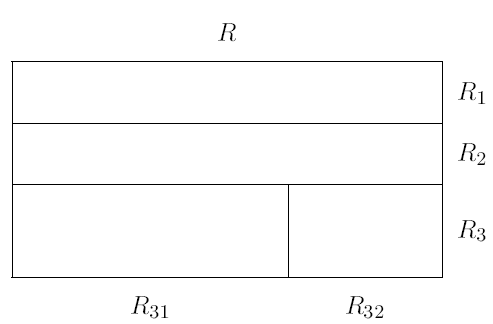
\includegraphics[scale=0.80]{Frag.png}
\caption{Hybride Fragmentierung}
\label{}
\end{figure}
\paragraph{Horizontale Fragmentierung\\\\}
Die horizontale Fragmentierung ist die in existierenden Systemen bedeutendste Fragmentierungsform und wird daher am ausführlichsten behandelt. Bei ihr wird eine globale Relation zeilenweise in disjunkte Teilmengen zerlegt. Die Zuordnung von Sätzen zu Fragmenten wird dabei i.a. über Selektionsprädikate definiert. Hierbei sind zwei Fälle zu unterscheiden. Bei der einfachen (primären) horizontalen Fragmentierung beziehen sich die Selektionsprädikate ausschließlich auf Attribute der zu zerlegenden Relation. Bei der abgeleiteten horizontalen Fragmentierung dagegen wird die Zerlegung auf die horizontale Fragmentierung einer anderen Relation abgestimmt.[Pic5]
\\\\
\newpage
\paragraph{Vertikale Fragmentierung\\\\}
Die vertikale Fragmentierung zerlegt eine Relation spaltenweise durch Definition von Projektionen auf den Attributen der Relation. Die Forderungen nach Vollständigkeit und Rekonstruierbarkeit verlangen, das jedes Attribut in wenigstens einem Fragment enthalten ist. Die Rekonstruktion der globalen Relation erfordert den natürlichen Verbund (Join) zwischen den einzelnen Fragmenten. Um diese Join-Berechnung verlustfrei vornehmen zu können, ist es jedoch erforderlich, den Primärschlüssel der globalen Relation (bzw. einen sonstigen Schlüsselkandidaten) in jedem Fragment mitzuführen. Die Forderung nach Disjunktheit muss also bei der vertikalen Fragmentierung auf die Nicht-Primärattribute (Attribute, die nicht Teil des Primärschlüssels sind) eingeschränkt werden.[Pic5]
\\
Die vertikale Fragmentierung kommt vor allem für Relationen mit einer großen Anzahl von Attributen zum Tragen, wenn an verschiedenen Knoten vorwiegend unterschiedliche Teilmengen der Attribute benötigt werden. In diesem Fall kann durch die vertikale Fragmentierung eine Reduzierung des Kommunikationsaufwandes erreicht werden sowie eine Einschränkung des zu verarbeitenden Datenumfanges. Auf der anderen Seite ist die Rekonstruktion der vollständigen Tupel über Verbunde teuer. \\Sehr aufwendig sind auch Änderungsvorgänge wie Einfügen oder Löschen von Tupeln, da sie sämtliche vertikalen Fragmente einer Relation betreffen.[Pic5]
\paragraph{Hybride Fragmentierung\\\\}
Da die Fragmente einer Relation selbst wiederum Relationen darstellen, kann die Fragmentierung rekursiv fortgesetzt werden, sofern die Korrektheit in jedem Fragmentierungsschritt gewahrt bleibt. Insbesondere können dabei die unterschiedlichen Fragmentierungsarten kombiniert werden, wobei man dann von einer hybriden Fragmentierung der globalen Relation spricht. Die Wiederherstellung einer derart zerlegten Relation erfordert die Ausführung der Rekonstruktionsschritte in der inversen Reihenfolge, in der die Fragmentierungen vorgenommen wurden.[Pic5]
\subsection{Synchronisation}
\subsubsection{Arten der Synchronisation}
\begin{figure}[hp]
\centering
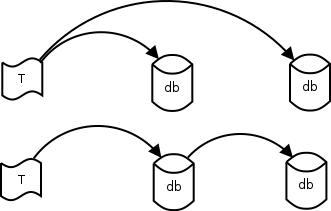
\includegraphics[scale=0.80]{syn.png}
\caption{Synchrone und Asynchrone Synchronisation}
\label{syn}
\end{figure}
\subsubsection{Synchron}
Tabellen die ständig geändert werden, müssen synchron gehalten werden. Hier besteht ebenfalls die Möglichkeit, die Replikate (mit Ausnahme eines, nämlich dem Original) nur für Lese-Zugriffe freizugeben. Damit ist die Synchronisation dann nur unidirektional durchzuführen. Die Daten des Replikats stehen dann wie oben nur zum Lesen zur Verfügung und alle Änderungen erfolgen auf dem Original. Dies ist aber nur dann sinnvoll, wenn die Änderungen hauptsächlich an einem Ort stattfinden und die Lesezugriffe über das Netzwerk zu zeitraubend sind. [Lau2]
\subsubsection{Asynchron}
Die asynchrone Replikation ist, wenn zwischen der Bearbeitung der primären Daten und den Replikaten eine Latenz vorliegt. Die Daten sind nur zum Zeitpunkt der Replikation synchron. Asynchrone Replikationsverfahren können mittels Read-Only oder Update-Anywhere realisiert werden. Bei Update-Everywhere kann auf allen Datenbanken geschrieben werden und es entsteht eine Aktualisierung in beide Richtungen. Bei Read-Only können die Daten nur von der primären Datenbank auf die Replizierten repliziert werden. [Lau2]
\subsection{Optimistische Synchronisation}
Optimistische Synchronisationsverfahren gehen von der Annahme aus, dass Konflikte zwischen Transaktionen seltene Ereignisse darstellen und somit das präventive Sperren der Objekte unnötigen Aufwand verursacht [KR81].  Daher wird ein nahezu beliebig paralleles Arbeiten auf der Datenbank erlaubt. Erst bei Transaktionsende wird überprüft, ob Konflikte mit anderen Transaktionen aufgetreten sind. Gemäß dieser Vorgehensweise unterteilt man die Ausführung einer Transaktion in drei Phasen:
\\\\
\emph{
In der Lesephase wird die eigentliche Transaktionsverarbeitung vorgenommen, d.h., es werden Objekte der Datenbank gelesen und modifiziert. Jede Transaktion führt dabei ihre Änderungen auf Kopien in einem ihr zugeordneten Transaktions-Puffer durch, der für keine andere Transaktion zugänglich ist.
\\\\
Bei EOT wird eine Validierungsphase gestartet, in der geprüft wird, ob die beendigungswillige Transaktion mit einer parallel zu ihr laufenden Transaktion in Konflikt geraten ist. Im Gegensatz zu Sperrverfahren, bei denen Blockierungen das primäre Mittel zur Behandlung von Synchronisationskonflikten sind, werden hier Konflikte stets durch Zurücksetzen einer oder mehrerer beteiligter Transaktionen aufgelöst. Es ist so zwar mit mehr Rücksetzungen als bei Sperrverfahren zu rechnen, dafür können aber bei optimistischen Verfahren keine Deadlocks entstehen.
\\\\
 Dies ist vor allem für Verteilte DBS ein potentieller Vorteil.
Die Schreibphase wird nur von Änderungstransaktionen ausgeführt, die die Validierungsphase erfolgreich beenden konnten. In dieser Phase wird zuerst die Wiederholbarkeit der Transaktion sichergestellt (Logging), bevor alle Änderungen durch Einbringen in die Datenbank für andere Transaktionen sichtbar gemacht werden. 
}
\subsection{Transaktionsmanagement}
In einer dezentralen Datenbank ist das Transaktionsmanagement sehr komplex, da bei einer globalen Transaktion nicht nur Daten auf einem Server geändert werden müssen, sondern auch auf Servern an anderen Standort, und sollte auch nur eine Teilaufgabe der Transaktion scheitern muss das ganze System zurückgesetzt werden um die Integrität der Datenbank zu erhalten. [Gei11]\\
Dadurch dass bei globalen Transaktionen Daten an mehreren Standorten geändert werden müssen ergeben sich dadurch einige Probleme. Schauen wir uns diese anhand eines Beispiels an:\\\\
Wir haben eine Bank mit mehreren Filialen (in ganz Österreich). Wir wollen Zinsen aller Kunden um 0.1 Prozent verringern. Dadurch wird ein \textbf{update} an alle Datenfragemente geschickt. Im Normalfall wird versucht die Tabelle Konto zu sperren, die Änderungen durchzuführen und dann die geänderten Daten zu \textbf{commit}en. Nehmen wir an das funktioniert ohne Probleme in allen Bundesländern außer Wien. In Wien kann die Tabelle nicht gesperrt werden und ein \textbf{rollback} wird erzwungen, und schon haben wir inkonsistente Daten verursacht.\\\\
Um solche Szenarien zu verhindert und um ein transparentes und vernünftiges Transaktionsmanagement zu haben ist es nötig ein Phasen-Commit-Protokoll zu implementieren.
\subsection{2 Phase Commit Protocol}
\begin{figure}[h]
\centering
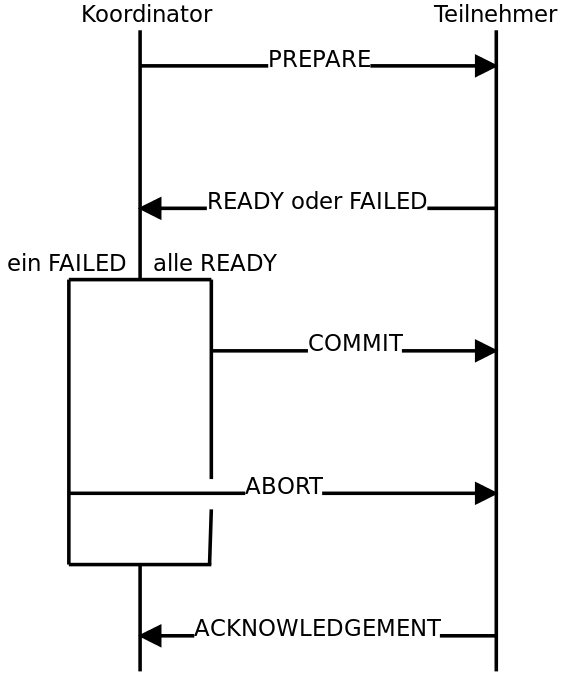
\includegraphics[scale=0.30]{Zwei_phasen_commit.png}
\caption{2-PC}
\label{2PC}
\end{figure}
Eine Lösung dafür ist das 2PC-Protokoll, welches auf dem Grundgedanken basiert, das alle an der Ausführung einer globalen Transaktion T beteiligten Knoten darüber abstimmen, ob T global commited werden darf, oder aborted wird. [Dad96]
\\\\
Die Phasen 2PC-Protokolls sind 'Prepare to Commit' und 'Commit/Abort'. In der ersten Phase werden alle Knoten aufgefordert den Commit der Transaktion vorzubereiten, also alle Änderungen zu sichern sowie ihre Stimme zu geben, ob T commited werden darf, oder nicht. [Kem6]
\\
In der zweiten Phase wertet der Koordinator des Commits (meist der Knoten, an dem T initiiert wurde) aus, ob der Commit stattfinden darf. Sobald ein einzelner Knoten mit 'abort' abstimmt, darf die Transaktion nicht commited werden, die Knoten müssen anschließend die Sperren auf alle Objekte von T lösen.Es gibt auch noch eine weiterentwickelte Form des 2PC-Protokolls, nämlich das 3PCProtokoll.[Kem6]
\\
Es funktioniert genau wie das 2PC-Protokoll, nur das eine Phase, in der abgefragt wird ob ein Commit überhaupt möglich ist, als erstes eingeschoben wird.
Mehr darüber nachlesen kann man in [Kem6].
\subsection{Mehrversionenkonzept}
Mehrversionen-Synchronisationsverfahren (multiversion concurrency control) streben eine Reduzierung an Synchronisationskonflikten an, indem für geänderte Objekte zeitweilig mehrere Versionen geführt werden und Leser ggf. auf ältere Versionen zugreifen. Voraussetzung dabei ist, daß für jede Transaktion vorab Wissen darüber vorliegt, ob sie möglicherweise Änderungen vornimmt.[Rah4]
\\
Einer reinen Lesetransaktion T wird dabei während ihrer gesamten Laufzeit eine Sicht auf die Datenbank gewährt, wie sie bei ihrem BOT gültig war; Änderungen, die während ihrer Bearbeitung vorgenommen werden, bleiben für T unsichtbar. [Rah4]
\\
Um dies zu realisieren, erzeugt jede erfolgreiche Änderung eine neue Version des modifizierten Objekts; die Versionen werden in einem sogenannten Versionen-Pool verwaltet. [Rah4]
\\
Im Gegensatz zu Lesetransaktionen greifen Änderungstransaktionen stets auf die aktuelle Version eines Objektes zu. Für ihre Synchronisation kann praktisch jedes der allgemeinen Synchronisationsverfahren verwendet werden [CM86, AS89].
\\\\
Da mit den Versionen jeder Lesetransaktion der bei BOT gültige (und konsistente) DB-Zustand zur Verfügung gestellt wird, ist für Lesetransaktionen keinerlei Synchronisation mehr erforderlich. Weiterhin brauchen sich andere Transaktionen nicht mehr gegen Lesetransaktionen zu synchronisieren.\\
Damit reduziert sich sowohl die Konfliktwahrscheinlichkeit (und damit die Anzahl von Blockierungen und Rücksetzungen) sowie der Synchronisierungsaufwand (Anzahl von Sperranforderungen, Validierungen etc.). Die Serialisierbarkeit bleibt generell gewahrt.
\subsection{Deadlocks}
Eine mit Sperrverfahren einhergehende Interferenz ist die Gefahr von Verklemmungen oder Deadlocks, deren charakterisierende Eigenschaft eine zyklische Wartebeziehung zwischen zwei oder mehr Transaktionen ist. Im verteilten Fall können diese Verklemmungen zwischen Transaktionen verschiedener Rechner auftreten, so dass es zu sogenannten globalen Deadlocks kommt.[Rah4]\\
Zur Deadlock-Behandlung in zentralisierten sowie in Verteilten DBS kommen einige generelle Strategien in Betracht: Verhütung, Vermeidung, Timeout, Erkennung sowie hybride Strategien. Diese Alternativen werden im Folgenden näher diskutiert. Besonderheiten für Verteilte DBS ergeben sich dabei vor allem bezüglich der Deadlock-Erkennung.[Rah4]\\
Die Deadlock-Verhütung (prevention) ist dadurch gekennzeichnet, dass die Entstehung von Deadlocks verhindert wird, ohne dass dazu irgendwelche Maßnahmen während der Abarbeitung der Transaktionen erforderlich sind. In diese Kategorie fallen v.a. die sogenannten Preclaiming-Sperrverfahren, bei denen eine Transaktion alle benötigten Sperren bereits bei BOT anfordern muss. Verklemmungen können dabei umgangen werden, indem jede Transaktion ihre Sperren in einer global festgelegten Reihenfolge anfordert, da dann keine zyklischen Wartebeziehungen entstehen können. Die eigentliche Ausführung einer Transaktion kann erst nach Erwerb aller benötigten Sperren beginnen, wobei im Fall von Sperrkonflikten die entsprechenden Wartezeiten in Kauf zu nehmen sind.[Rah4]
\\
Ein wesentliches Problem der Deadlock-Verhütung ist, dass bei Beginn einer Transaktion i.a. nur Obermengen der zu referenzierenden Objekte (z.B. ganze Relationen) bekannt sind. Der somit verursachte Grad an Sperrkonflikten ist daher in der Regel inakzeptabel. Dies gilt umso mehr, da die Sperren während der gesamten Transaktionslaufzeit zu halten sind. Im verteilten Fall kommt als weiterer Nachteil hinzu, dass für nicht lokal verwaltete Objekte vor Transaktionsbeginn eigene Kommunikationsvorgänge für die Sperranforderungen erforderlich sind.\\
Wegen dieser Schwächen hat der Preclaiming-Ansatz keine praktische Relevanz für Datenbanksysteme. Wir gehen daher im Weiteren bei Sperrverfahren davon aus, dass die Sperren während der Transaktionsverarbeitung (unmittelbar vor einem Objektzugriff) angefordert werden.[Rah4]
\newpage

\bibliographystyle{unsrt}
\bibliography{Synchronisierung_Konsistenz_Braendli_Weinb_5BHIT}
\begin{tabular}{ll}
	{[AS89]} & D. Agrawal \& S. Sengupta. Modular Synchronization in Multiversion Databases\\
	{[CM86]} & M.J. Carey \& W.A. Muhanna. The Performance of Multiversion Concurrency Control Algorithms. 1986. \\
	{[Gei1]} & Frank Geisler. Datenbanken Grundlagen und Design. 2011.\\
	{[Kem6]} & Alfons Kemper, André Eickler. Datenbanksysteme. 2006.\\
	{[Lau2]} & F. Laux. Verteilte datenbanken. 2002.\\
	{[Pic5]} & Reinhard Pichler. Verteilte Datenbanken. 2015.\\
	{[Rah4]} & Erhard Rahm. Grundlagen der verteilten und parallelen Datenbankverarbeitung. 1994.\\	
\end{tabular}

\listoffigures

\end{document}
